
\documentclass[%
pdftex,
oneside,			% Einseitiger Druck.
11pt,				% Schriftgroesse
parskip=half,		% Halbe Zeile Abstand zwischen Absätzen.
%	topmargin = 10pt,	% Abstand Seitenrand (Std:1in) zu Kopfzeile [laut log: unused]
headheight = 12pt,	% Höhe der Kopfzeile
%	headsep = 30pt,	% Abstand zwischen Kopfzeile und Text Body  [laut log: unused]
headsepline,		% Linie nach Kopfzeile.
footsepline,		% Linie vor Fusszeile.
footheight = 16pt,	% Höhe der Fusszeile
abstracton,		% Abstract Überschriften
DIV=calc,		% Satzspiegel berechnen
BCOR=8mm,		% Bindekorrektur links: 8mm
headinclude=false,	% Kopfzeile nicht in den Satzspiegel einbeziehen
footinclude=false,	% Fußzeile nicht in den Satzspiegel einbeziehen
listof=totoc,		% Abbildungs-/ Tabellenverzeichnis im Inhaltsverzeichnis darstellen
toc=bibliography,	% Literaturverzeichnis im Inhaltsverzeichnis darstellen
]{scrreprt}	% Koma-Script report-Klasse, fuer laengere Bachelorarbeiten alternativ auch: scrbook


\def \titel {Erarbeitungs-/Reflexionsphase -- Entwicklung eines real-time Backends für eine datenintensive Applikation}
\def \arbeit {Seminararbeit}
\def \autor {Jasper Bremenkamp}
\def \abschluss {Master of Science}
\def \studiengang {Data Science}
\def \datumAbgabe {\today}
\def \modul {Projekt: Data Engineering}
\def \matrikelnr {92125193}
\def \tutor {Prof. Dr. Max Pumperla}

\def \seitenrand {2cm}

% PDF Einstellungen
\usepackage{hyperref}

\hypersetup{
    unicode = true,
    pdftitle={\titel},
    pdfauthor={\autor},
    pdfsubject={\arbeit},
    pdfcreator={pdflatex, LaTeX with KOMA-Script},
    pdfpagemode=UseOutlines, 		% Beim Oeffnen Inhaltsverzeichnis anzeigen
    pdfdisplaydoctitle=true, 		% Dokumenttitel statt Dateiname anzeigen.
    pdflang={de}, 			% Sprache des Dokuments.
    hidelinks
}

\usepackage[left=2cm,right=2cm,top=2cm,bottom=2cm]{geometry} % margins	% Seitenränder und Abstände
\usepackage[activate]{microtype} %Zeilenumbruch und mehr
\usepackage[onehalfspacing]{setspace}
\usepackage{makeidx}
\usepackage[autostyle=true,german=quotes]{csquotes}
\MakeOuterQuote{"} % Für deutsche Anführungszeichen
\usepackage{longtable}
\usepackage{enumitem}	% mehr Optionen bei Aufzählungen
\usepackage{graphicx}
\usepackage{pdfpages}   % zum Einbinden von PDFs
\usepackage{xcolor} 	% für HTML-Notation
\usepackage{float}
\usepackage{array}
\usepackage{calc}		% zum Rechnen (Bildtabelle in Deckblatt)
\usepackage[right]{eurosym}
\usepackage{wrapfig}
\usepackage{pgffor} % für automatische Kapiteldateieinbindung
\usepackage[perpage, hang, multiple, stable]{footmisc} % Fussnoten
\usepackage[printonlyused]{acronym} % falls gewünscht kann die Option footnote eingefügt werden, dann wird die Erklärung nicht inline sondern in einer Fußnote dargestellt
\usepackage{listings}
\usepackage{bookmark}
\usepackage[english, ngerman]{babel}
\usepackage[utf8]{inputenc}
\usepackage{scrhack}
\usepackage{dirtree}
\usepackage{txfonts} % Use a Times-new-roman open-source clone


    %%%%%%% Neues Design %%%%%%%%%%%
    \setkomafont{chapter}{\Large}
    \setkomafont{section}{\large}
    \setkomafont{subsection}{\large}

    %\renewcommand*\chapterheadstartvskip{\vspace*{-0cm}} %Kapitel nach oben verschieben

    \addtolength{\footskip}{-0.7cm}% foot larger by 0,7 cm  (Raises the page number)
    \setlength{\parindent}{6pt} % Indent at start of paragraphs  6pt

    \renewcommand\thesection{\arabic{section}}
    \renewcommand\thefigure{\arabic{figure}}

    %%%%%%%%%%%%%%%%%%%%%%%%%%%%%%%

% Notizen. Einsatz mit \todo{Notiz} oder \todo[inline]{Notiz}.
\usepackage[obeyFinal,backgroundcolor=yellow,linecolor=black]{todonotes}
% Alle Notizen ausblenden mit der Option "final" in \documentclass[...] oder durch das auskommentieren folgender Zeile
% \usepackage[disable]{todonotes}

% Kommentarumgebung. Einsatz mit \comment{}. Alle Kommentare ausblenden mit dem Auskommentieren der folgenden und dem aktivieren der nächsten Zeile.
\newcommand{\comment}[1]{\par {\bfseries \color{blue} #1 \par}} %Kommentar anzeigen

% der neue Zitierstil ist Käse
\global\def\VAlterZitierstil{true}

\global\def\VTrueValue{true}

\ifx\VAlterZitierstil\VTrueValue
    \usepackage[
        backend=bibtex,     % empfohlen. Falls biber Probleme macht: bibtex
        bibwarn=true,
        bibencoding=utf8,   % wenn .bib in utf8, sonst ascii
        sortlocale=de_DE,
        sorting=none,
        style=numeric-comp
    ]{biblatex}

    \addbibresource{bibliographie.bib}
\else
    % New IUBH Cite Style / Old Cite style below
    \usepackage{natbib}
    \setcitestyle{aysep={}} % remove comma as delimiter
\fi


\begin{document}

\pagenumbering{Roman}

\begin{titlepage}
    \pdfbookmark{\titel}{}
    \begin{longtable}{p{7cm} p{12cm}}
        {\raisebox{\ht\strutbox-\totalheight}{
\includegraphics[height=3cm]{assets/iu.png}}}
    \end{longtable}
    \enlargethispage{20mm}
    \begin{center}
        \vspace*{12mm}	{\LARGE\textbf \titel }\\
        \vspace*{12mm}	{\large\textbf \arbeit}\\
        \vspace*{12mm}	Prüfungsleistung für den\\
        \vspace*{3mm}		{\textbf \abschluss}\\
        \vspace*{12mm}	des Studiengangs \studiengang\\
    \vspace*{3mm}		an der Internationalen Hochschule\\
        \vspace*{12mm}	von\\
        \vspace*{3mm}		{\large\textbf \autor}\\
        \vspace*{12mm}	\datumAbgabe
    \end{center}
    \vfill
    \begin{spacing}{1.2}
    \begin{tabbing}
        mmmmmmmmmmmmmmmmmmmmmmmmmm             \= \kill
        \textbf{Kursbezeichnung} \> \modul\\
        \textbf{Matrikelnummer} \> \matrikelnr\\
        \textbf{Tutor} \> \tutor\\
    \end{tabbing}
    \end{spacing}
\end{titlepage}

\newpage

%Abbildungsverzeichnis
%\cleardoublepage %To-Do: Wieder hinzufügen, wenn sinnvolle Grafiken eingefügt werden
%\listoffigures

%Tabellenverzeichnis
%\cleardoublepage
%\listoftables

%\chapter{Konzeption} %evtl weg lassen und section sind dann chapter
\pagenumbering{arabic}

% \comment{Inhalt: \\
% Beschreibung des Hintergrund-Szenarios \\
% Dokumentierung von Informationslücken \\
% Strategie zur Beschaffung/Füllung der Informationslücken \\
% }

% \comment{Anforderungen: \\
% Nicht mehr als 2 Seiten
% Diagramme und Schaubilder nach Ermessen einsetzbar
% }

\section{Implementierung}

    Die Umsetzung der Dateninfrastruktur basiert auf einer modularen Microservice-Architektur, die für die Echtzeitverarbeitung großer Datenmengen entwickelt wurde.
    Die Architektur fokussiert sich auf Zuverlässigkeit, Skalierbarkeit und Wartbarkeit, während sie gleichzeitig datenschutzrechtliche Anforderungen erfüllt.

    Eine Visualisierung ist in nachfolgender Abbildung \ref{fig:architekturentwurf} zu sehen.

    \begin{figure}[H] %To-Do: Grafik evtl weiter konkretisieren. Bisher nur Kopie aus der Konzeptionsphase
        \centering
        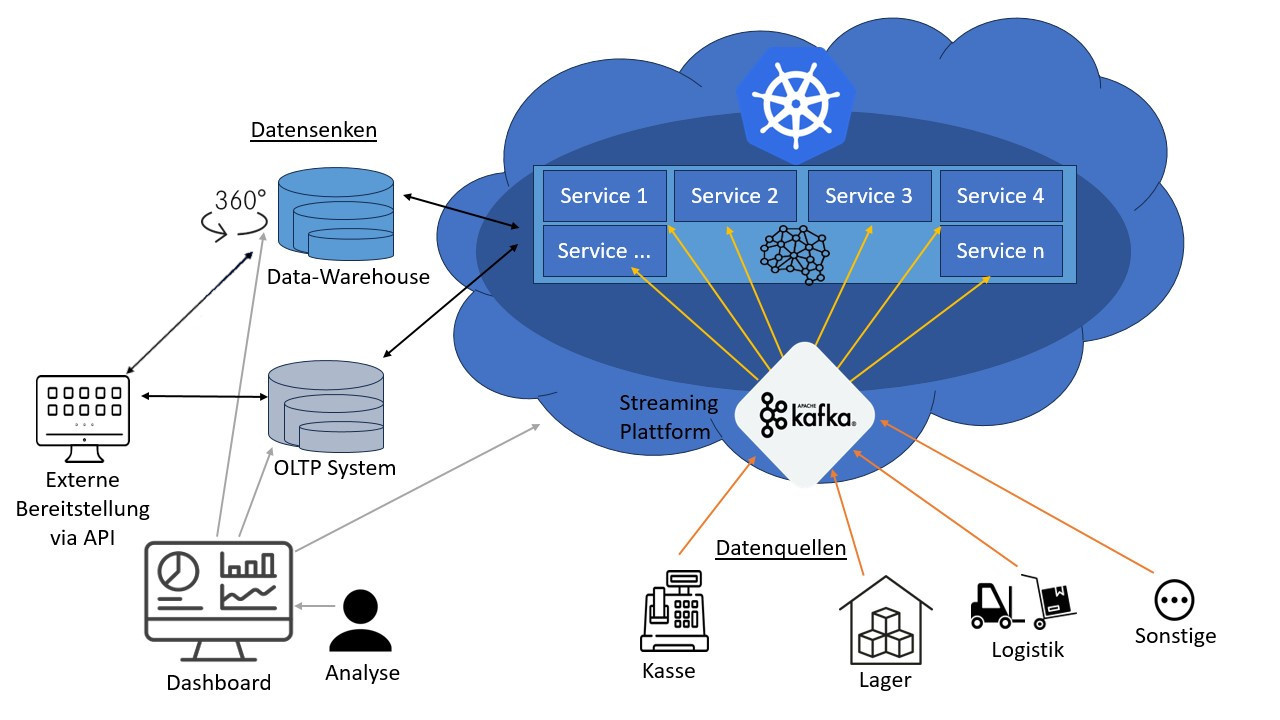
\includegraphics[width=1\textwidth]{assets/architekturentwurf.jpg}
        \caption{Architekturübersicht}
        \label{fig:architekturentwurf}
    \end{figure}

    Zur Datenaufnahme, Verarbeitung und Kommunikation zwischen den Komponenten werden ausschließlich Python-Microservices eingesetzt.
    Jeder Microservice ist so konzipiert, dass er eine klar definierte Aufgabe erfüllt und unabhängig von anderen Services agieren kann.
    Die Kommunikation erfolgt über Apache Kafka, das als Message-Broker verwendet wird.
    Die Daten werden in Kafka Topics geschrieben, von den zuständigen Microservices konsumiert und anschließend verarbeitet.
    Dabei wird keine zusätzliche Middleware wie Kafka Streams genutzt, sondern die gesamte Datenlogik ist direkt in den Python-Microservices implementiert.

    Mehrere Microservices übernehmen die Aufgabe Datenströme zu simulieren, die Verkaufs- und Bestandsdaten repräsentieren.
    Im Produktivbetrieb würden dise Microservices echte Daten aus den Fillialen und Lagerhäuser als Edge Nodes verarbeiten und an Kafka übergeben.
    Diese Daten werden direkt an Kafka Topics publiziert.
    Die simulierten Daten dienen als Testbasis, um die Funktionalität der gesamten Pipeline unter realistischen Bedingungen zu validieren.
    Weitere spezialisierte Microservices konsumieren diese Daten und führen Tranformationen durch, wie etwa Aggregationen und das Extrahieren relevanter Informationen.
    Die Aggregationen erfolgen in zeitlich definierten Intervallen, um Echtzeitberichte bereitzustellen.

    Die stark konsuldierten und zu persistierenden Daten werden in einer PostgreSQL-Datenbank gespeichert, die für eine effiziente Speicherung und Abfrage großer Datenmengen optimiert ist.
    Die Übergabe der Daten an die Datenbank erfolgt durch einen dedizierten Microservice, der die Daten aus Kafka konsumiert, verarbeitet und in die entsprechenden Tabellen einfügt.
    Diese Struktur ermöglicht eine klare Trennung der Verantwortlichkeiten zwischen Datenaufnahme, Verarbeitung und Speicherung.

    Kubernetes wird zur Orchestrierung der Microservices genutzt.
    Die Bereitstellung und Konfiguration der Services erfolgt über Helm-Charts, die eine einfache Verwaltung und Skalierung der Infrastruktur gewährleisten.
    Dies ermöglicht es, die Infrastruktur flexibel an veränderte Anforderungen, wie etwa größere Datenvolumina, anzupassen.

    Besonderer Wert wird auf Datensicherheit und Datenschutz gelegt.
    Die Kommunikation zwischen den Microservices wird im Produktivbetrieb verschlüsselt erfolgen, und rollenbasierte Zugriffskontrollen (RBAC) stellen sicher, dass nur autorisierte Entitäten Zugriff auf die Daten haben. %Nochmal erläutern und ggf. verfizieren
    Schützenswerte Daten, die nicht persistiert werden müssen, werden durch die Kafka Retention automatisch innerhalb kürzerer Zeit gelöscht und müssen nicht gesondert im Rahmen der DSGVO behandelt werden.
    Zudem werden alle Datenflüsse umfassend dokumentiert, um den Richtlinien der Datenschutz-Grundverordnung (DSGVO) zu entsprechen.
    Für die persistenten Daten und die Einhaltung der DSGVO gibt es speziell einen Microservice, der die Aufgabe der Einhaltung übernimmt.

    Der Quellcode der Infrastruktur, der Applikationen inkl. der Dokumentation wird in einem Git-Repository versioniert, um die Nachvollziehbarkeit und Reproduzierbarkeit sicherzustellen.
    Das Repository enthält alle relevanten Konfigurationsdateien, Python-Skripte und Helm-Charts, die für den Aufbau der Infrastruktur notwendig sind.

    Das Repository ist über folgenden Link zugänglich:
    \url{https://github.com/jasper-bk/Projekt_DataEngineering_WiSe2024-2025}. %To-Do: Sicherstellen, dass der Link auch verfügbar ist oder ggf. durch einen anderen Link ersetzen

    Erste Tests zeigen, dass das System in der Lage ist, große Datenmengen effizient zu verarbeiten und in Echtzeit bereitzustellen.
    Die Architektur erfüllt die Anforderungen an Zuverlässigkeit, Skalierbarkeit und Wartbarkeit und stellt eine robuste Grundlage für zukünftige Erweiterungen dar.
    Das Optimierungspotenzial liegt insbesondere in der Ressourcennutzung des Kubernetes-Clusters, um die Performance weiter zu verbessern.

% To-Dos:
% Nochmal klären, ob auch hier mehr als eine halbe Seite Okay ist.
% Code noch sinnvoll finalisieren. Tabellen werden nur bedingt genutzt und die "Business"-Logik selbst ist noch fraglich
%   - Evtl auch klären wie wichtig die Logik selbst ist, ob z. B. auch Platzhalter zulässig sind
% Generell klären, wie umfangreich der Text für die zweite Phase sein soll.
%   - Falls mehr Details erwünsch sind, dann auch mehr auf den Code, die Topics und den Aufbau des Helm-Charts eingehen
% Thema Datensicherheit und Datenschutz besser fokussieren oder zumindest klären ... Wie viel ist wirklich schon notwendig. Reichen auch Platzhalter? DSGVO Microservice z. B. ...

%Folgende Fragen klären:
% TBD

\ifx\VAlterZitierstil\VTrueValue
    \printbibliography
\else
    \bibliographystyle{iubh}
    \bibliography{bibliographie.bib}
\fi
\end{document}
